\documentclass{ltjsarticle}
\usepackage{amsmath}
\usepackage{amssymb}
\usepackage{ascmac}
\usepackage[dvipdfmx]{graphicx}
\usepackage[colorlinks=true, allcolors=blue]{hyperref}
\usepackage{fancybox}
\usepackage{tikz}
\usepackage{subcaption}
\usetikzlibrary{shapes,arrows}

\begin{document}

\title{深層学習 day2}
\author{秋葉洋哉}
\maketitle

\section{ニューラルネットワーク}
\subsection{勾配消失問題}
\begin{figure}[htbp]
  \centering
  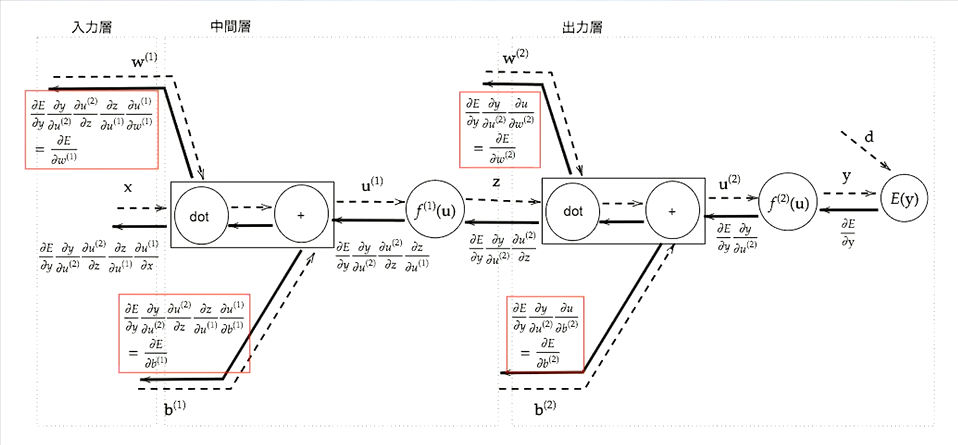
\includegraphics[width=13cm]{./capture/backprop.png}
  \caption{誤差逆伝播法における勾配}
  \label{fig:backprop}
\end{figure}
勾配消失問題とは、多層ニューラルネットワークにおいて、勾配が逆伝播する際に、勾配が小さくなり、学習が進まなくなる問題である。
勾配消失問題は、シグモイド関数やハイパボリックタンジェント関数を活性化関数として用いた場合に発生しやすい。
シグモイド関数の微分は、
\begin{align}
  \frac{d}{dx}\sigma(x) = \sigma(x)(1 - \sigma(x))
\end{align}
であり、これをグラフにすると、最大値が0.25であることがわかる。
図\ref{fig:backprop}において、活性化関数$f(u)$をシグモイド関数として考えた時、$u$の更新式である、
\begin{align}
  u^{(3)} &\leftarrow u - \epsilon \frac{\partial E}{\partial y}\frac{\partial y}{\partial u}\\
  u^{(2)} &\leftarrow u - \epsilon \frac{\partial E}{\partial y}\frac{\partial y}{\partial u^{(3)}} \frac{\partial u^{(3)}}{\partial z^{(2)}} \frac{\partial z^{(2)}}{\partial u^{(2)}}\\
  u^{(1)} &\leftarrow u - \epsilon \frac{\partial E}{\partial y} \frac{\partial y}{\partial u^{(3)}} \frac{\partial u^{(3)}}{\partial z^{(2)}} \frac{\partial z^{(2)}}{\partial u^{(2)}} \frac{\partial u^{(2)}}{\partial z^{(1)}} \frac{\partial z^{(1)}}{\partial u^{(1)}}
\end{align}
における、$\frac{\partial y}{\partial u}, \frac{\partial z^{(2)}}{\partial u^{(2)}}, \frac{\partial z^{(1)}}{\partial u^{(1)}}$が最大値0.25の少数となる。模式図では中間層が1層のみであるが、実際にはさらに多くの層を持つため、これらの値が掛け合わされることで、勾配が指数関数的に小さくなり、勾配消失問題が発生する。
\par
勾配消失問題に対しては以下の3つの解決方法が考えられる。
\begin{enumerate}
  \item 活性化関数の選択
  \item 重みの初期値の設定
  \item バッチ正規化
\end{enumerate}

\subsubsection{活性化関数の選択}
活性化関数の選択については、ReLU関数やLeaky ReLU関数を用いることで、勾配消失問題を回避することができる。
Leaky ReLU関数は以下の数式で定義される。
\begin{align}
  f(x) = \begin{cases}
    x & (x > 0)\\
    ax & (x \leq 0)
  \end{cases}
\end{align}
ここで、$a$は0より大きい小さな値である。
Leaky ReLU関数は、$x \leq 0$の時に、勾配が0にならず、$x$に比例して勾配が変化するため、勾配消失問題を回避することができる。
ReLU関数は、微分値が1になるため先ほどのシグモイド関数における問題が解消される (図\ref{fig:LeakyReLU})。

最近では、Swish関数といった活性化関数も提案されている。Swish関数は以下の数式で定義される。
\begin{align}
  f(x) &= x \cdot \sigma(\beta x)\\
  \frac{\partial}{\partial x}f(x) &= \beta f(x) + \sigma(\beta x) (1 - \beta f(x))
\end{align}
ここで、$\sigma$はシグモイド関数であり、$\beta$はハイパーパラメータである。
Swish関数は、ReLU関数を滑らかにしたものであり、ReLU関数よりも高い性能を発揮することが報告されている(図\ref{fig:Swish})。

\begin{figure}[ht]
  \centering
  \begin{subfigure}[b]{0.45\textwidth}
    \centering
    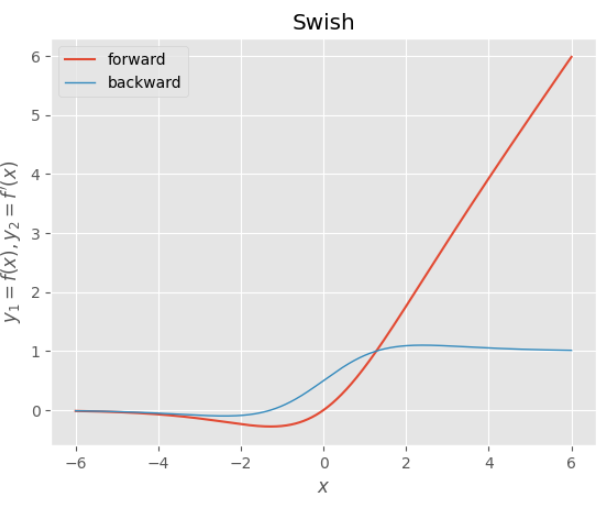
\includegraphics[width=\textwidth]{./capture/Swish.png}
    \caption{Swish関数のグラフ}
    \label{fig:Swish}
  \end{subfigure}
  \hfill
  \begin{subfigure}[b]{0.45\textwidth}
    \centering
    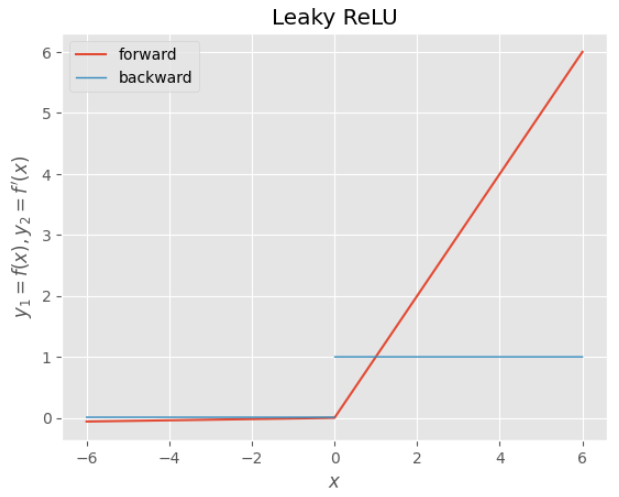
\includegraphics[width=\textwidth]{./capture/LeakyReLU.png}
    \caption{LeakyReLU関数のグラフ}
    \label{fig:LeakyReLU}
  \end{subfigure}
  \caption{}
\end{figure}

\subsubsection{重みの初期値設定}
重みの初期値の設定については、活性化関数がsigmoidやtanhの場合Xavierの初期値、活性化関数がReLUの場合Heの初期値を用いることで、勾配消失を抑制することができる。
\par
Xavierの初期値は、前の層のノード数を$n$とした時、標準偏差が$\frac{1}{\sqrt{n}}$の分布を用いて、対象の層と前の層の間の重みを初期化する方法である。
\par
Heの初期値は、前の層のノード数を$n$とした時、標準偏差が$\frac{2}{\sqrt{n}}$の分布を用いて、対象の層と前の層の間の重みを初期化する方法である。
\subsubsection{バッチ正規化}
バッチ正規化は、最初の入力データの正規化だけでなく、各層の出力に対しても正規化することで、勾配消失問題を回避して汎化性能を上げる方法である(図\ref{fig:Batch_Normalization})。
バッチ正規化は、学習時と推論時で挙動が異なるため、学習時には、ミニバッチごとに正規化を行い、推論時には、全データを用いて正規化を行う必要がある。
バッチ正規化を行う際は、まずミニバッチの平均・分散を求める。
\begin{align}
  \mu_i &= \frac{1}{m}\sum_{i=1}^{m}x_i \text{  (平均)} \\
  \sigma_i^2 &= \frac{1}{m}\sum_{i=1}^{m}(x_i - \mu_i)^2 \text{  (分散)}
\end{align}
次に、正規化を行う。この時、$\epsilon$を加えることで、分母が0になるのを防ぐ。
\begin{align}
  \hat{x}_i &=\frac{\text{(各値の平均からの差)}}{\text{(標準偏差)}}\\
  &=  \frac{x_i - \mu_i}{\sqrt{\sigma_i^2 + \epsilon}} 
\end{align}
最後に、スケーリングとシフトを行う。
\begin{align} 
  y_i = \gamma \hat{x}_i + \beta
\end{align}
ここで、$\gamma$はスケーリング係数、$\beta$はシフト係数、$\epsilon$は微小値である。

\begin{itembox}[l]{正規化の種類}
  バッチ正規化には、他にも以下のような正規化手法がある。
  \begin{itemize}
    \item レイヤー正規化 (図\ref{fig:Layer_Normalization})
    \item インスタンス正規化 (図\ref{fig:Instance_Normalization})
    \item グループ正規化 (図\ref{fig:Group_Normalization})
  \end{itemize}
\end{itembox}

\begin{figure}[htbp]
  \centering
  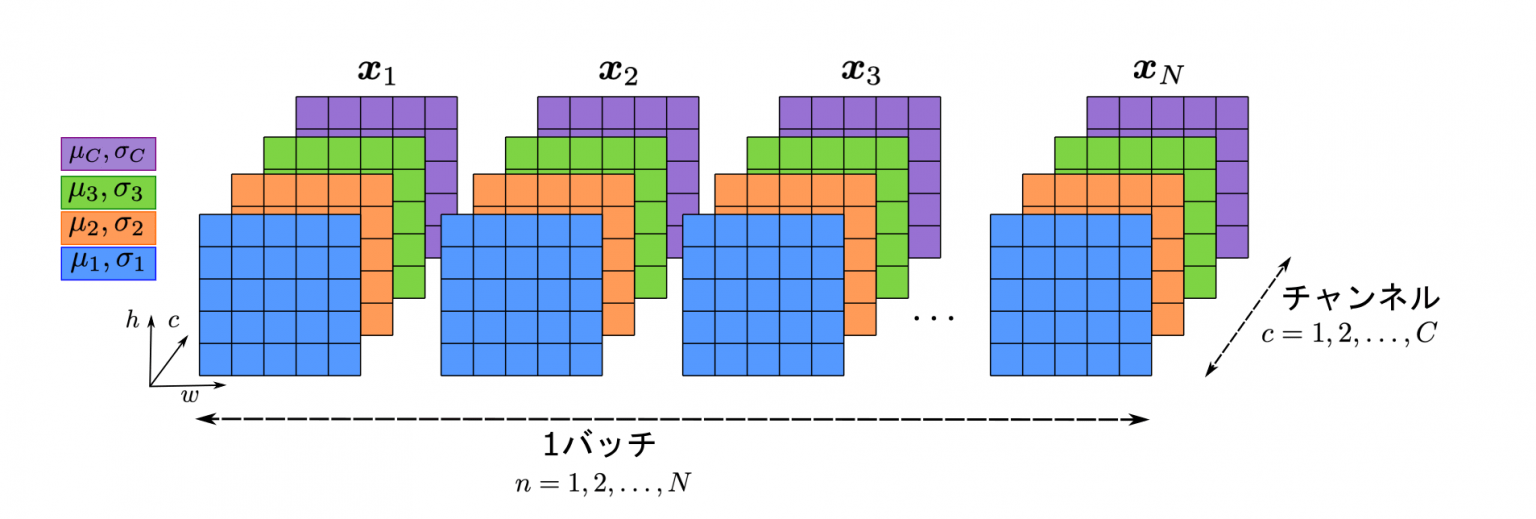
\includegraphics[width=10cm]{./capture/Batch_Normalization.png}
  \caption{バッチ正規化のイメージ: バッチ内全体で、チャンネル単位の正規化を行う。(https://cvml-expertguide.net/terms/dl/layers/batch-normalization-layer/ より引用)}
  \label{fig:Batch_Normalization}
\end{figure}

\begin{figure}[htbp]
  \centering
  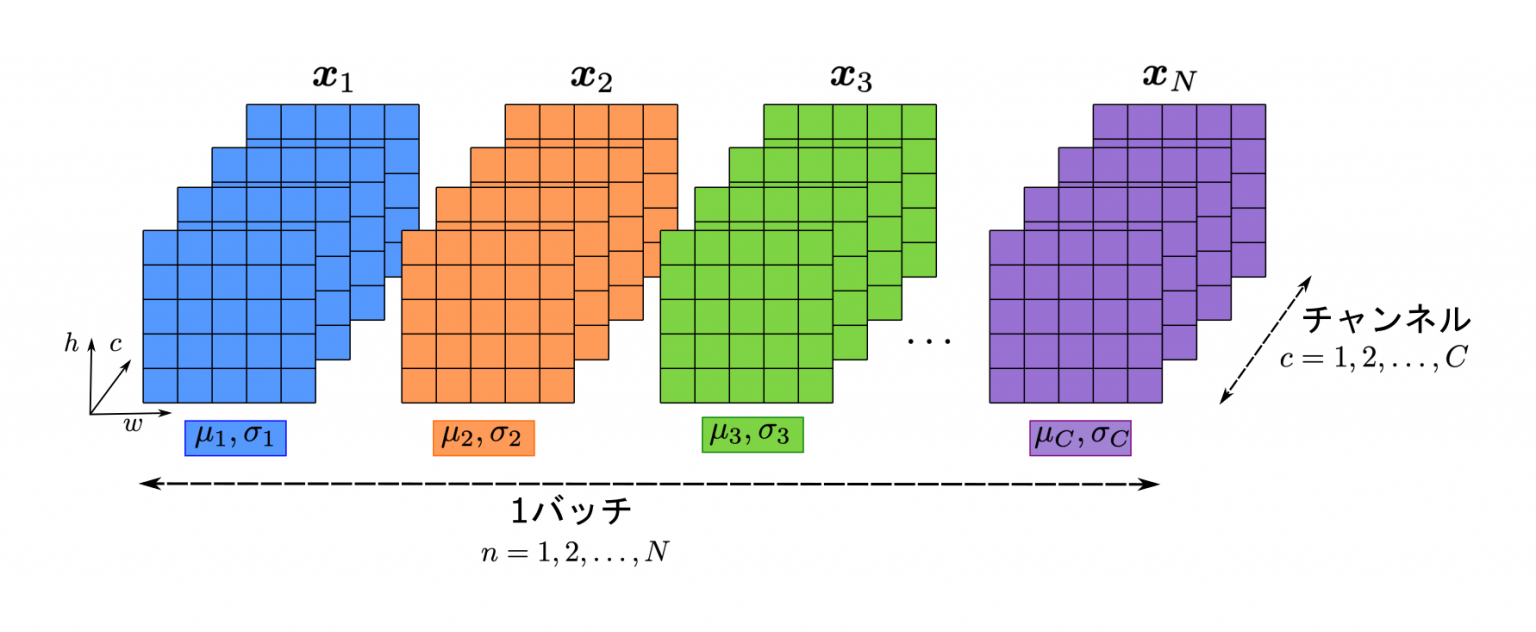
\includegraphics[width=10cm]{./capture/Layer_Normalization.png}
  \caption{レイヤー正規化のイメージ: チャンネル内全体で、層単位の正規化を行う。(https://cvml-expertguide.net/terms/dl/layers/batch-normalization-layer/ より引用)}
  \label{fig:Layer_Normalization}
\end{figure}

\begin{figure}[htbp]
  \centering
  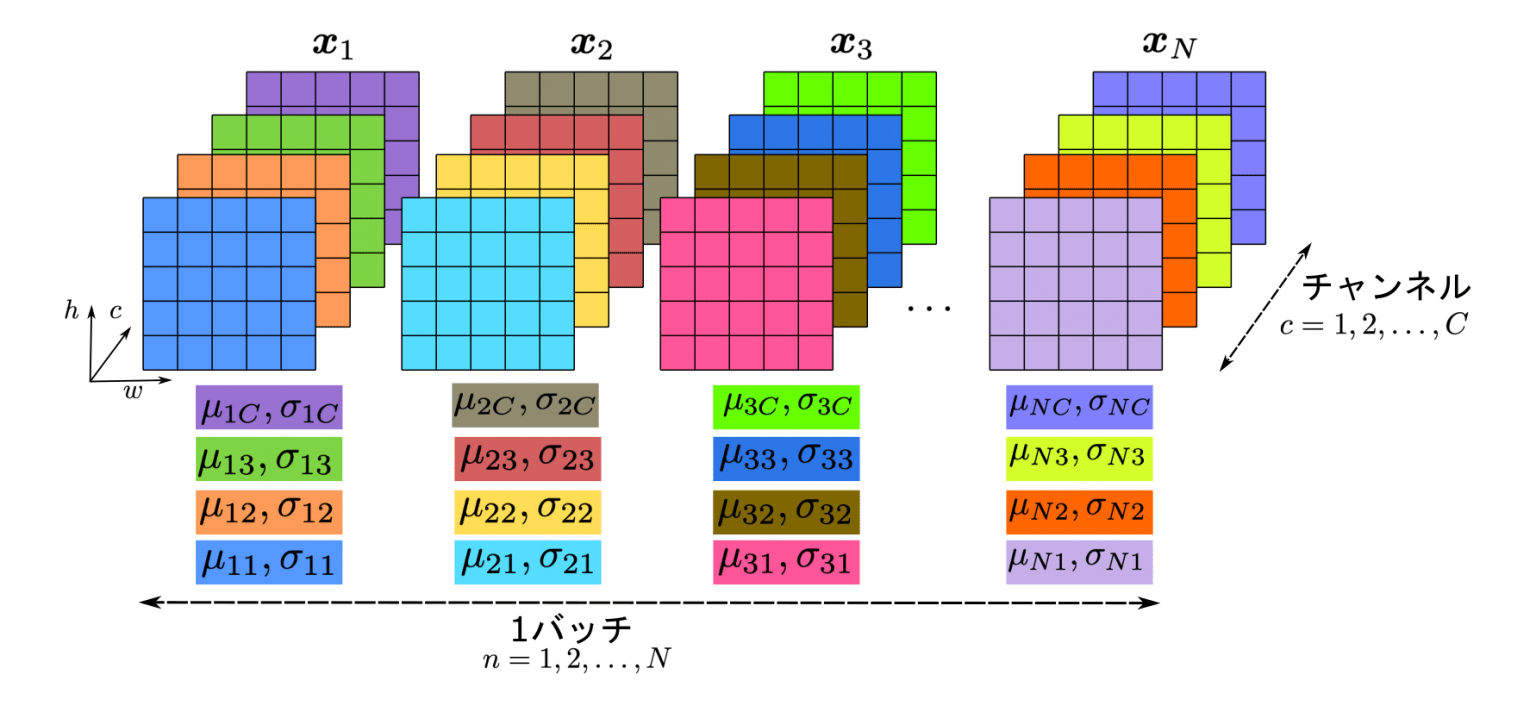
\includegraphics[width=10cm]{./capture/Instance_Normalization.png}
  \caption{インスタンス正規化のイメージ: 画像一枚単位で、チャンネル毎の正規化を行う。(https://cvml-expertguide.net/terms/dl/layers/batch-normalization-layer/ より引用)}
  \label{fig:Instance_Normalization}
\end{figure}

\begin{figure}[htbp]
  \centering
  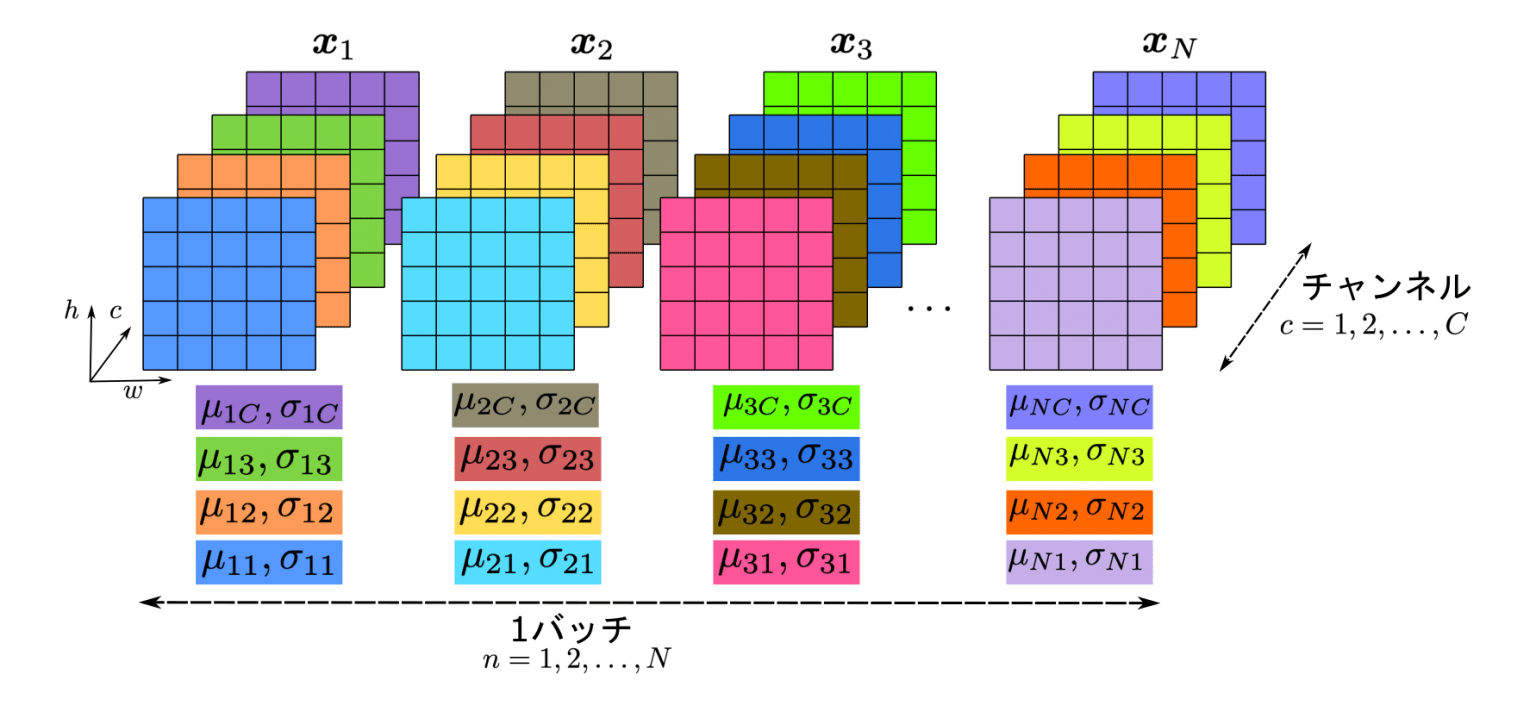
\includegraphics[width=10cm]{./capture/Instance_Normalization.png}
  \caption{グループ正規化のイメージ: 各1サンプル内のグループ単位で正規化を行う。(https://cvml-expertguide.net/terms/dl/layers/batch-normalization-layer/ より引用)}
  \label{fig:Group_Normalization}
\end{figure}




\begin{itembox}[l]{確認テスト}
  Q: 重みの初期値を0に設定すると、どのような問題が発生するか。簡潔に説明せよ。

  A: 順伝播での出力がすべて同じ値となり、逆伝搬での勾配もすべて同じ値となるため、重みの更新がうまく行われず、学習が進まなくなる。

  Q: 一般的に考えられるバッチ正規化の効果を2点挙げよ。

  A: 学習データとテストデータの分布が異なる場合に、評価値を安定させる効果がある (汎化性能が上昇する)。また、勾配消失を解消して学習を早く進めることができる。
\end{itembox}



\subsection{学習率最適化手法}
学習率最適化手法とは、学習率を適切に設定するための手法である。学習率とは、重みの更新量を調整するためのハイパーパラメータであり、大きすぎると発散し、小さすぎると収束が遅くなるため、適切な値を設定する必要がある。
学習率最適化手法には、以下のような手法がある。
\begin{enumerate}
  \item Momentum
  \item AdaGrad
  \item RMSProp
  \item Adam
\end{enumerate}

\subsubsection{Momentum}
Momentumは、勾配方向に加えて、前回の重みの更新量を考慮して、重みを更新する手法である。
Momentumは、以下の式で表される。
\begin{align}
  v^{(t+1)} &= \epsilon \frac{\partial E}{\partial w} - \mu v^{(t)} \\
  w^{(t+1)} &= w^{(t)} - v^{(t+1)}
\end{align}
ただし、$\epsilon$は学習率、$\mu$はモメンタムと呼ばれるハイパーパラメータである。
前回の重みの更新量に$\mu = 0.5 \sim 0.9$の値を掛け合わせたもの$v$を更新量として用いることで、勾配降下法における振動を抑える。よって、大域的最適解に向かって、谷の方向に沿って谷底を効率よく探索して収束していく特徴がある。

\subsubsection{AdaGrad(Adaptive Gradient Algorithm)}
AdaGradは、学習率を重みの要素ごとに変化させる手法である。
これまでの勾配の二乗和を経験としてすべて保持し、その経験に基づいて学習率を調整する。
AdaGradは、以下の式で表される。
\begin{align}
  h^{(t+1)} &= h^{(t)} + \left( \frac{\partial E}{\partial w} \right)^2 \\
  w^{(t+1)} &= w^{(t)} - \frac{\epsilon}{\sqrt{h^{(t+1)}}} \frac{\partial E}{\partial w}
\end{align}
ただし、$h$はこれまでの勾配の二乗和を保持する変数である。
AdaGradは、学習率が小さくなりすぎるという問題がある。
確かに、誤差関数の勾配が大きい場合、2つ目の式で、$\frac{1}{\sqrt{h^{(t+1)}}}$によって更新量が小さくなることが分かる。これを改善したものがRMSPropである。


\subsubsection{RMSProp}
RMSPropは、AdaGradの学習率が小さくなりすぎる問題を解決するために、指数移動平均を用いて、過去の勾配の影響を減衰させる手法である。
つまり、過去の経験を忘れることで、学習率が小さくなりすぎる問題を解決するということである。
RMSPropは、以下の式で表される。
\begin{align}
  h^{(t+1)} &= \alpha h^{(t)} + (1 - \alpha) \left( \frac{\partial E}{\partial w} \right)^2 \\
  w^{(t+1)} &= w^{(t)} - \frac{\epsilon}{\sqrt{h^{(t+1)}}} \frac{\partial E}{\partial w}
\end{align}
ここで、$\alpha$は減衰率を表すハイパーパラメータである。
RMSPropは、AdaGradの学習率が小さくなりすぎる問題を解決するが、逆に学習率が大きくなりすぎる問題がある。
Adamはこれを解決するために提案された。

\subsubsection{Adam}
Adamは、Momentumの過去の勾配の指数関数的減衰平均と、RMSPropの二乗和の移動平均を組み合わせた手法である。
Adamは、以下の式で表される。
\begin{align}
  m^{(t+1)} &= \beta_1 m^{(t)} + (1 - \beta_1) \frac{\partial E}{\partial w} \\
  h^{(t+1)} &= \beta_2 h^{(t)} + (1 - \beta_2) \left( \frac{\partial E}{\partial w} \right)^2 \\
  \label{eq3}
  \hat{m} &= \frac{m^{(t+1)}}{1 - \beta_1^{t+1}} \\
  \label{eq4}
  \hat{h} &= \frac{h^{(t+1)}}{1 - \beta_2^{t+1}} \\
  w^{(t+1)} &= w^{(t)} - \frac{\epsilon}{\sqrt{\hat{h}} + \epsilon} \hat{m}
\end{align}
ここで、$\beta_1, \beta_2$はそれぞれMomentumとRMSPropの減衰率を表すハイパーパラメータである。式\eqref{eq3}と式\eqref{eq4}は、バイアス補正を行うための式で、$\beta$の肩の数字は乗算を表す。


\subsection{過学習}
過学習とは、学習データに対しては良い性能を示すが、テストデータに対しては性能が低くなる現象である。
深層学習モデルにおいて過学習が発生する原因は、以下の3つが挙げられる。
\begin{itemize}
  \item パラメータ数が多い
  \item データが少ない
  \item ノード数が多い
  \item → ネットワークの自由度が高いということ
\end{itemize}
過学習では、重みの行列の中で、極端に大きな値を持つものが現れてしまうことによって発生する。
過学習を防ぐためには、以下のような手法がある。
\begin{enumerate}
  \item 正則化
  \item ドロップアウト
  \item 早期終了
  \item データ拡張
\end{enumerate}

\subsubsection{正則化}
正則化は、過学習を防ぐために、誤差関数に正則化項を追加する手法である。
一般化されたL(N)正則化項は、以下の式で表される。
\begin{align}
  E(\mathbf{w}) + \frac{1}{p} \lambda ||\mathbf{w}||_p \\
  ||\mathbf{w}||_p = \left( \sum_{i=1}^{n}|w_i|^p \right)^{\frac{1}{p}}
\end{align}
ここで、$\lambda$は正則化項の重みを表すハイパーパラメータである。 
L1正則化は、$p=1$の場合であり、L2正則化は、$p=2$の場合である。
例えば、xとyの2次元のデータがある場合、L1正則化は、
\begin{align}
  |x| + |y|
\end{align}
となり、L2正則化は、
\begin{align}
  \sqrt{x^2 + y^2}
\end{align}
となる。
\begin{figure}
  \centering
  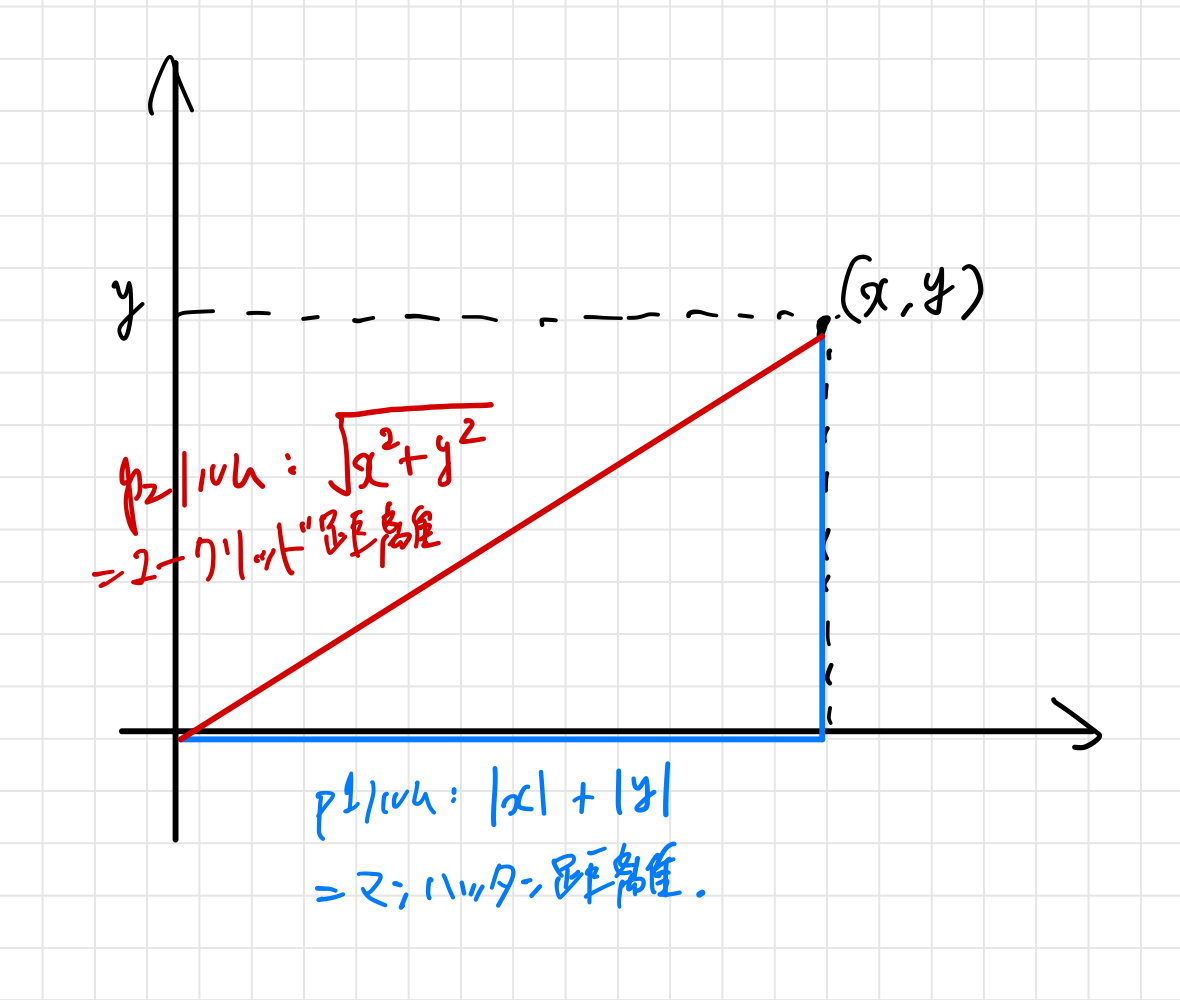
\includegraphics[width=10cm]{./capture/L1L2.png}
  \caption{L1, L2ノルムのイメージ}
\end{figure}
L1正則化を用いた回帰分析のことをLasso回帰と呼ぶ。Lasso回帰は、L1正則化を用いることで、スパースな解を得られやすいため、必要な特徴量のみを選択することができる (図\ref{fig:Lasso}) 。
L2正則化を用いた回帰分析のことをRidge回帰と呼ぶ。Ridge回帰は、L2正則化を用いることで、特徴量の重みを0に近づけることができるため、特徴量の重みを抑制することができる (図\ref{fig:Ridge}) 。

\begin{figure}[ht]
  \centering
  \begin{subfigure}[b]{0.45\textwidth}
    \centering
    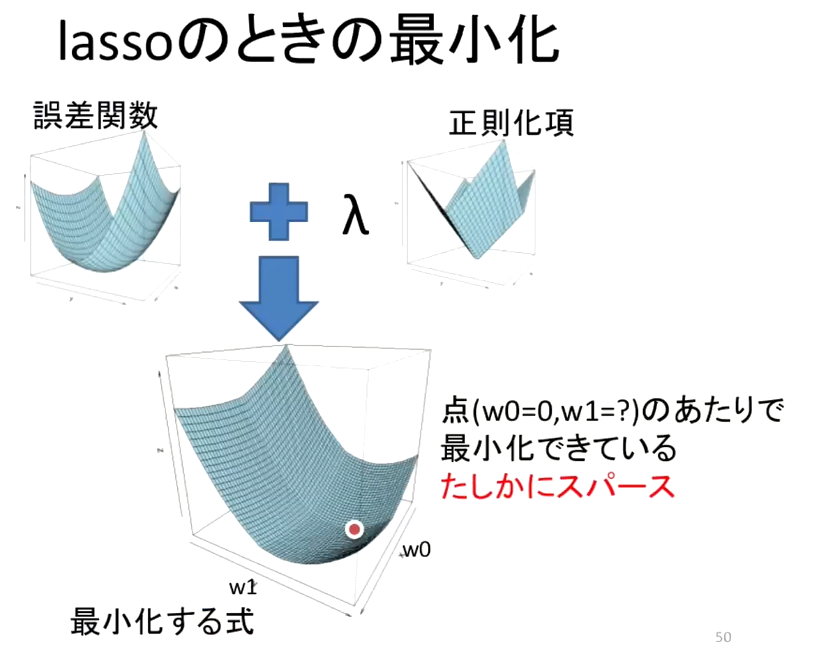
\includegraphics[width=\textwidth]{./capture/Lasso.png}
    \caption{Lasso回帰における正則化のイメージ (参照: 授業資料(Day2 18 過学習 正則化手法4))}
    \label{fig:Lasso}
  \end{subfigure}
  \hfill
  \begin{subfigure}[b]{0.45\textwidth}
    \centering
    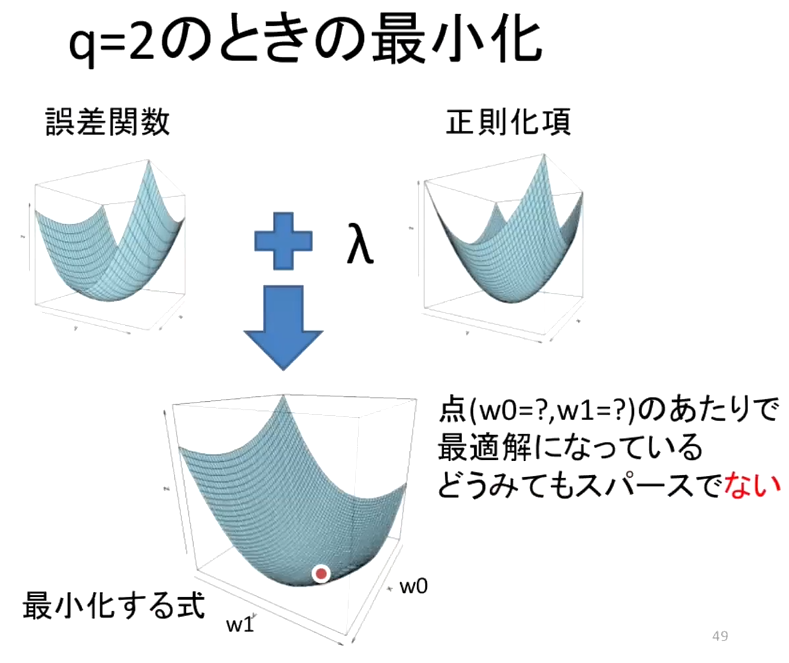
\includegraphics[width=\textwidth]{./capture/Ridge.png}
    \caption{Ridge回帰における正則化のイメージ (参照: 授業資料 Day2 18 過学習 正則化手法4))}
    \label{fig:Ridge}
  \end{subfigure}
  \caption{}
\end{figure}

\begin{itembox}[l]{Pythonコード}
それぞれの正則化手法を用いた場合の重みの更新量は以下の通りである。

\begin{verbatim}
  # L2正則化
    for idx in range(1, hidden_layer_num + 1): 
      # 重みの勾配([Afiine + str(idx)].dW)に、正則化強度(weight_decay_lambda)*重み([params + str(idx)])を加算する
      grad['W' + str(idx)] = network.layers['Affine' + str(idx)].dW + weight_decay_lambda * network.params['W' + str(idx)]
      # 重みの更新量(network.params['W' + str(idx)]) = 学習率(learning_rate) * 重みの勾配(grad['W' + str(idx)])
      network.params['W' + str(idx)] -= learning_rate * grad['W' + str(idx)]

      # バイアスに正則化は適用しない
      grad['b' + str(idx)] = network.layers['Affine' + str(idx)].db
      network.params['b' + str(idx)] -= learning_rate * grad['b' + str(idx)]

      # 重みの更新量の二乗和平方(np.sqrt(np.sum(network.params['W' + str(idx)] ** 2)))
      # 重みの更新量の二乗和平方に正則化強度*0.5を掛けたものを weight_decay に加算して更新する。
      weight_decay += 0.5 * weight_decay_lambda * np.sqrt(np.sum(network.params['W' + str(idx)] ** 2))

    # 損失関数に weight_decay を加算する
    loss = network.loss(x_batch, d_batch) + weight_decay

  # L1正則化
    for idx in range(1, hidden_layer_num+1):
      grad['W' + str(idx)] = network.layers['Affine' + str(idx)].dW + weight_decay_lambda * np.sign(network.params['W' + str(idx)])
      grad['b' + str(idx)] = network.layers['Affine' + str(idx)].db
      network.params['W' + str(idx)] -= learning_rate * grad['W' + str(idx)]
      network.params['b' + str(idx)] -= learning_rate * grad['b' + str(idx)]
      # L1正則化の場合は、重みの更新量の絶対値の和を weight_decay に加算して更新する。
      weight_decay += weight_decay_lambda * np.sum(np.abs(network.params['W' + str(idx)]))
    
    loss = network.loss(x_batch, d_batch) + weight_decay

loss = network.loss(x_batch, d_batch) + weight_decay
\end{verbatim}
\end{itembox}


\begin{itembox}[l]{確認テスト}
  Q: 図\ref{fig:day2_18_1}について、L1正則化を表しているグラフはどちらか答えよ。

  A: 順伝播での出力がすべて同じ値となり、逆伝搬での勾配もすべて同じ値となるため、重みの更新がうまく行われず、学習が進まなくなる。
\end{itembox}

\begin{figure}
  \centering
  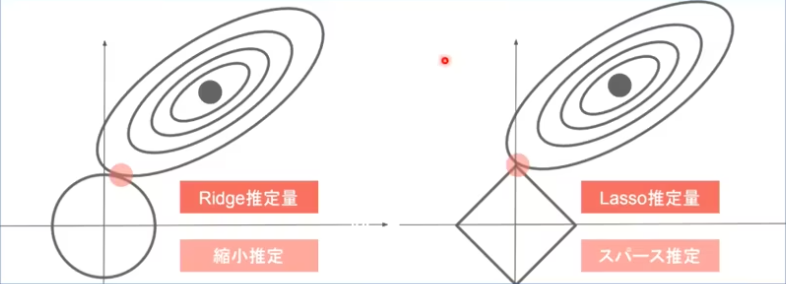
\includegraphics[width=10cm]{./capture/confirm_test/day2_18_1.png}
  \caption{}
  \label{fig:day2_18_1}
\end{figure}



\subsubsection{ドロップアウト}
ドロップアウトは、ニューラルネットワークの学習時に、ランダムにノードを削除することで、過学習を防ぐ手法である。
ドロップアウトは、以下の式で表される。
\begin{align}
  y_i = r_i \times x_i
\end{align}
ここで、$r_i$は、ノード$i$を削除する確率を表すハイパーパラメータである。
ドロップアウトは、学習時にのみ適用し、テスト時には適用しない。
ドロップアウトは、モデルの自由度を下げることで、過学習を防ぐ効果がある。


\newpage
\section{畳み込みニューラルネットワーク(CNN)}
\subsection{概要}
CNNは、画像認識や音声認識などの分野で高い性能を発揮するニューラルネットワークである。
ある画像に対しては、隣り合うピクセルの情報が似通う可能性が高い。また、ある動画に対しては、連続するフレームの画像情報が似通う可能性が高い。
そのような次元間で連続した情報を扱う際に、CNNは高い効果を発揮する。

\subsection{LeNet}
LeNetは、畳み込みニューラルネットワークの元祖とも言われるモデルである。CNNを理解するために、まずはLeNetの構造について説明する。
LeNetにおける入力層は、32x32の画像、つまり1024の数字の集まりであり、畳み込み層を通過することで、画像の特徴を10種類に分類、つまり10の数字に絞り込む。
LeNetでは、特徴マップである畳み込み層と、その要約としてのプーリング層を交互に繰り返すことで、画像の特徴を抽出している。
その過程は以下の通りである。図\ref{fig:lenet}は、LeNetの概要を示している。
\begin{enumerate}
  \item 入力層: 32x32の画像
  \item C1: 畳み込み層 (28×28×6通りの特徴マップ) を生成
  \item S2: プーリング層 (14×14×6通りの特徴マップ) に要約
  \item C3: 6つの特徴マップを基に畳み込み層 (10×10×16通りの特徴マップ) を生成
  \item S4: プーリング層 (5×5×16通りの特徴マップ) に要約
  \item C5: 全結合層 (120通りの特徴マップ) を生成
  \item F6: 全結合層 (84通りの特徴マップ) を生成
  \item 出力層→ 10種類の数字に分類
\end{enumerate}

  \begin{figure}[htbp]
    \centering
    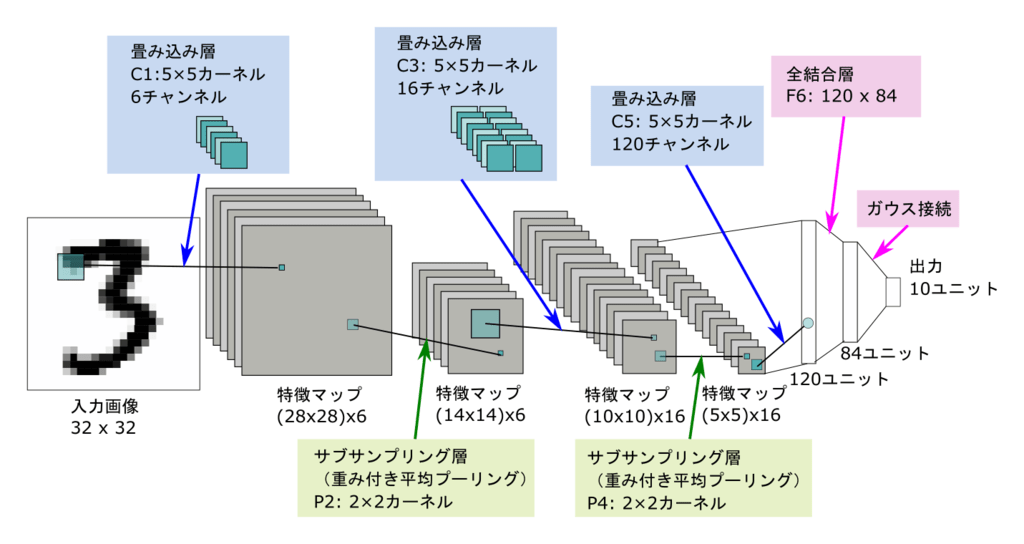
\includegraphics[width=14cm]{./capture/LeNet.png}
    \caption{LeNetの概要(https://cvml-expertguide.net/terms/dl/cnn/cnn-backbone/lenet/より引用)}
    \label{fig:lenet}
\end{figure}
  
\newpage

\subsection{畳み込み(Convolution)層}
\begin{figure}
  \centering
  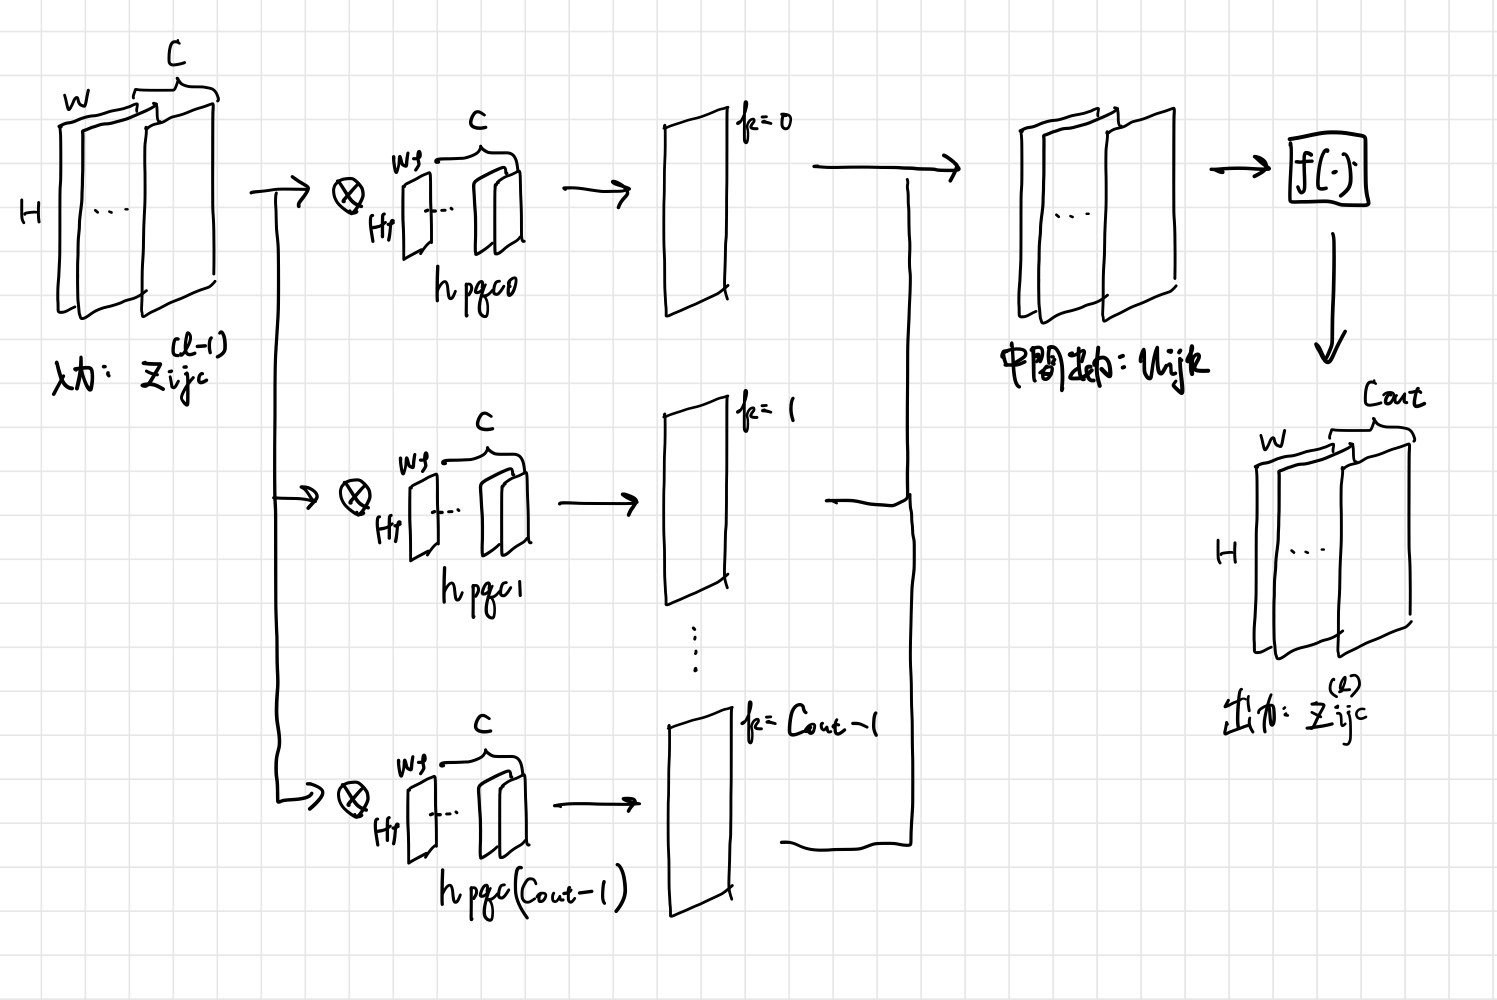
\includegraphics[width=12cm]{./capture/Convolution_layer.png}
  \caption{畳み込み層の概念図. この畳み込み層は$W\times H \times C$の入力に対し、$C_{\text{out}}$個のフィルタ(縦横 $W_f\times H_f \times C$)を適用し、$W\times H \times C_{\text{out}}$の出力を得る.}
  \label{fig:convolution_layer}
\end{figure}
CNNでは、LeNet同様、畳み込み層、プーリング層、全結合層から構成される。
CNNにおける畳み込み層では、フィルタ(カーネルとも呼ぶ)を用いて、画像という大きな行列の特徴を抽出する。
フィルタは、画像の一部分に対して「重みのかけ合わせ = 畳み込み」を行い、画像の特徴を抽出するための行列である。
\par
第$l-1$層から$W \times H\times C$の入力$z_{ijc}^{(l-1)}$を受け取り、$C_{\text{out}}$種類のフィルタ$h_{pqck}(k=0, \cdots, C_{\text{out}}-1)$を適用する場合を考える(図\ref{fig:convolution_layer})。各フィルタのチャネル数は入力と同じ数$C$であり、フィルタのサイズは$W_f \times H_f \times C$と書ける。1種類のフィルタに着目すると、入力チャンネル1つに対して、$W \times H \times 1$の出力を得る。これをすべてのチャンネルで計算を行うと、$W \times H \times C$の出力を得る。この出力をチャンネル方向で足し合わせて、1種類のフィルタに対して、$W \times H \times 1$の出力を得る。ここまでの計算は、以下で表すことができる。
\begin{align}
  u_{ijk}^{(l)} = \sum_{c=0}^{C-1}\sum_{p=0}^{W_f-1}\sum_{q=0}^{H_f-1}z_{i+p, j+q, c}^{(l-1)}h_{pqck} + b_k
\end{align}
$u_{ijk}^{(l)}$は、$k$番目のフィルタに対する出力である。ただし、$b_k$はバイアスである。この計算をすべてのフィルタに対して行うことで、$W \times H \times C_{\text{out}}$の出力を得ることができる。この出力を活性化関数に通して、最終的な出力$z_{ijk}^{(l)}$を得る。

\par
この積和演算を画像に対して行うことで、画像の特徴を抽出することができる。
畳み込みでは、次元の繋がりを保ちながら、画像の特徴を抽出するために、フィルタをスライドさせて、画像全体に対して演算を行う。フィルタの数は、画像の特徴を抽出するための次元数であり、フィルタの数が多いほど、画像の特徴を多く抽出することができる。
\par
畳み込み層における主要なハイパーパラメータには、以下のようなものがある。
\begin{itemize}
  \item パディング
  \item ストライド
  \item チャンネル
\end{itemize}
\par
パディングは、画像の次元を保つために画像の端にハイパーパラメータを追加することである。
パディングを行うことで、フィルタのサイズ分小さくなる画像のサイズを元のサイズのまま保つことができる。
\par
ストライドは、フィルタをスライドさせる幅を表すハイパーパラメータである。
ストライドを大きくすることで、画像の次元を小さくすることができる。
\par
チャンネルは、フィルタの数を表すハイパーパラメータである。
チャンネルを増やすことで、画像の特徴を多く抽出することができる。



\begin{itembox}[l]{確認テスト}
  Q: サイズ6×6の入力画像を、サイズ2×2のフィルタで畳み込んだ時の出力画像のサイズを答えよ。なおストライドとパディングは1とする。
 
  A: 出力画像は5×5となる。なぜなら、ストライド1の時、フィルタをスライドさせる間隔は1つずつで、パディングが1の時、入力画像の周囲に1マスずつ余白が生じるためである。\\
  なお、公式は以下の通りとなる。

  \begin{align}
    \frac{{\text{入力画像のサイズ}} + 2 \times \text{パディング} - \text{フィルタサイズ}}{{\text{ストライド}}} + 1
  \end{align}
 
\end{itembox}

\subsection{プーリング(pooling)層}
一般的にプーリング層では2つの役割がある。1つは、入力の各位置でその局所領域内の値を要約することであり、もうひとつは入力の空間解像度を下げるダウンサンプリングの実行である。
要約の仕方は、畳み込んだ行列の中で最大の値を取り出したり、平均値を取り出すなどがある。
この時、前者の方法をMaxプーリング、 後者の方法をAverageプーリングと呼ぶ。


\subsection{全結合層}
全結合層は、畳み込み層やプーリング層で抽出した特徴を元に、最終的な出力を行う層である。
全結合層では、畳み込み層やプーリング層で抽出した特徴を1次元のベクトルに変換し、出力層に渡す。
数式では単にアフィン変換を行うだけであるが、この層がないと、畳み込み層やプーリング層で抽出した特徴を元に、最終的な出力を行うことができない。
\begin{align}
  \mathbf{y} = \mathbf{W} \mathbf{x} + \mathbf{b}
\end{align}
全結合層はしばしば線形層、Linearクラスまたは単にLinearと記述されることが多い。
\par
1次元への変換は、Flatten, Global MaxPooging, Global AveragePoolingなどの手法がある。
Flattenは、抽出した特徴をすべて1次元のベクトルに変換する手法である
Global MaxPoolingは、抽出した特徴の中から1チャンネルの中での最大の値を取り出す手法である。
Global AveragePoolingは、抽出した特徴の中から1チャンネルの中での平均値を取り出す手法である。


\subsection{AlexNet}
AlexNetは、深層学習による画像認識ブームの火付け役となったモデルである。
224×224の画像を入力とし、55×55の畳み込み層、27×27のプーリング層、13×13の畳み込み層、6×6のプーリング層、全結合層、出力層から構成される。
AlexNetでは、以下の工夫を行ったことで、誤差が大幅に削減され、高い性能を発揮した。
\begin{enumerate}
  \item ReLU関数の導入
  \item ドロップアウトの導入
  \item データ拡張
  \item バッチ正規化
\end{enumerate}

それまでのCNNでは、シグモイド関数やハイパボリックタンジェント関数を活性化関数として用いていたが、これらの関数を用いた場合、層を増やした時に微分値が小さくなるため、勾配が爆発したり消失する問題があった。
ReLU関数は、そのような問題を解決するために導入された関数であり、勾配が消失しないため、層を深くすることができた。

\subsection{GoogLeNet}
GoogLeNetは、2014年に発表されたモデルであり、当時としてはとても層が多く、深いネットワークを有するモデルであった。その深いネットワークを実現するために、様々な問題を回避しつつ、層数を増やした点が現代においても評価されている。
以下に、その工夫点を示す。
\begin{enumerate}
  \item Inceptionモジュールの導入
  \item Auxilary Lossの導入
  \item Alobal Average Poolingの導入
\end{enumerate}

\subsubsection{Inceptionモジュール}
Inceptionモジュールでは、異なるフィルタサイズを持つ畳み込み層を並列に組み合わせることで、層を深くすることなくフィルターの種類を増やすことができる。フィルターの種類を増やすことで、異なる空間分解能で特徴抽出を行うので、より性能の高いモデルを構築することができる。
1×1の畳み込み層は、Pointwise Convolutionと呼ばれ、次元削減を行うために用いられる。入力のチャンネル数よりも少ない種類のフィルターを用いることで、チャンネル方向でまとめられた特徴をフィルターの数分出力することができる。
\begin{figure}[ht]
  \centering
  \begin{subfigure}[b]{0.45\textwidth}
    \centering
    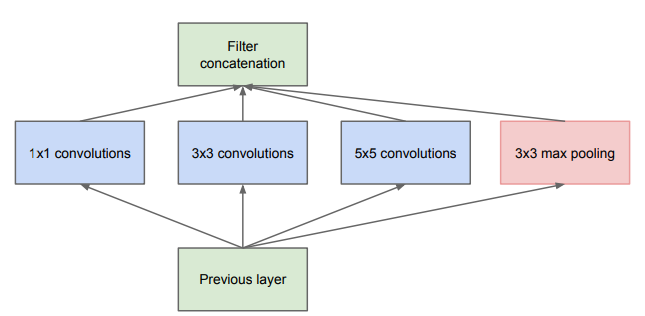
\includegraphics[width=\textwidth]{./capture/GoogLeNet_Inception_Naive.png}
    \caption{シンプルなInceptionモジュール (出典: https://arxiv.org/pdf/1409.4842)}
    \label{fig:Inception_Naive}
  \end{subfigure}
  \hfill
  \begin{subfigure}[b]{0.45\textwidth}
    \centering
    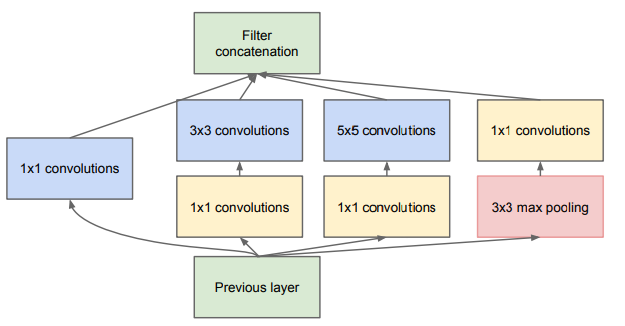
\includegraphics[width=\textwidth]{./capture/GoogLeNet_Inception_dimension_reductions.png}
    \caption{次元削減を伴うInceptionモジュール (出典: https://arxiv.org/pdf/1409.4842)}
    \label{fig:Inception_dimension_reductions}
  \end{subfigure}
  \caption{Inceptionモジュールの概略図}
\end{figure}

\subsubsection{Auxilary Loss}
Auxilary Lossは、GoogLeNetにおいて、途中の層で出力を行い、その出力に対して損失関数を適用する手法である。この手法は、勾配消失問題を回避するために導入された手法であり、途中の層で出力を行うことで、途中の層での勾配が消失することを防ぐことができる。

\subsubsection{Global Average Pooling}
Global Average Poolingは、畳み込み層やプーリング層で抽出した特徴を、チャンネル方向に平均を取る手法である。この手法は、畳み込み層やプーリング層で抽出した特徴を1次元のベクトルに変換することができるため、全結合層に入力することができる。


\paragraph{参考文献}
\begin{enumerate}
  \item 岡谷貴之/深層学習 改訂第2版 [機械学習プロフェッショナルシリーズ]/ 講談社サイエンティフィク/ 2022-01-17
  \item バッチ正規化 (Batch Normalization) とその発展形 \url{https://cvml-expertguide.net/terms/dl/layers/batch-normalization-layer/}
  \item 全結合層 (fully-connected layer) [線形層] \url{https://cvml-expertguide.net/terms/dl/layers/fully-connected-layer/}
  \item LeNet: 最初のCNN構造 \url{https://cvml-expertguide.net/terms/dl/cnn/cnn-backbone/lenet/}
  \item AlexNet: 大規模な画像物体認識むけCNNの元祖 \url{https://cvml-expertguide.net/terms/dl/cnn/cnn-backbone/alexnet/#3_AlexNet_\%E3\%81\%AE\%E7\%89\%B9\%E5\%BE\%B4\%E3\%83\%BB\%E5\%B7\%A5\%E5\%A4\%AB}
  \item 【要点を整理】GoogleNetをわかりやすく解説 \url{https://dx-consultant-fast-evolving.com/googlenet/}
  \item Going deeper with convolutions \url{https://arxiv.org/pdf/1409.4842}
\end{enumerate}

\end{document}